\documentclass[a4paper,11pt]{article}
\usepackage{amssymb, enumitem}
\setlist[enumerate,1]{label={\bfseries\arabic*.},ref={\bfseries{Ejercicio \arabic*}}}
\setlist[enumerate,2]{label={\bfseries(\alph*)},ref={\bfseries(\alph*)}}


\parindent 0cm
\usepackage{amssymb,amsmath,amsthm,latexsym,epsfig,euscript,multicol}
\usepackage{graphbox}
\usepackage{booktabs}

\usepackage[utf8x]{inputenc}
\usepackage{listings,xcolor,bm}
\usepackage{url}
\usepackage{hyperref}
\hypersetup{
    colorlinks=true,
    urlcolor=blue,
    }


\definecolor{mygreen}{rgb}{0,0.6,0}
\definecolor{mygray}{rgb}{0.5,0.5,0.5}
\definecolor{mymauve}{rgb}{0.58,0,0.82}
\lstset{
  backgroundcolor=\color{white},   % choose the background color; you must add
  basicstyle=\ttfamily,      % the size of the fonts that are used for the code
  breakatwhitespace=true,         % sets if automatic breaks should only happen at whitespace
  breaklines=true,                 % sets automatic line breaking
  captionpos=b,                    % sets the caption-position to bottom
  commentstyle=\color{mygreen},    % comment style
  deletekeywords={...},            % if you want to delete keywords from the given language
  escapeinside={\%*}{*)},          % if you want to add LaTeX within your code
  extendedchars=true,              % lets you use non-ASCII characters; for 8-bits encodings only, does not work with UTF-8
  firstnumber=1,                % start line enumeration with line 1000
  frame=none,	                   % adds a frame around the code
  keepspaces=true,                 % keeps spaces in text, useful for keeping indentation of code (possibly needs columns=flexible)
  keywordstyle=\color{blue},       % keyword style
  language=Python,                 % the language of the code
  morekeywords={*,...},            % if you want to add more keywords to the set
  numbers=none,                    % where to put the line-numbers; possible values are (none, left, right)
  numbersep=5pt,                   % how far the line-numbers are from the code
  numberstyle=\tiny\color{mygray}, % the style that is used for the line-numbers
  rulecolor=\color{black},         % if not set, the frame-color may be changed on line-breaks within not-black text (e.g. comments (green here))
  showspaces=false,                % show spaces everywhere adding particular underscores; it overrides 'showstringspaces'
  showstringspaces=false,          % underline spaces within strings only
  showtabs=false,                  % show tabs within strings adding particular underscores
  stepnumber=5,                    % the step between two line-numbers. If it's 1, each line will be numbered
  stringstyle=\color{mymauve},     % string literal style
  tabsize=4,	                   % sets default tabsize to 2 spaces
  title=\lstname,                  % show the filename of files included with \lstinputlisting; also try caption instead of title
  belowskip=0em
}
% Caracteres especiales
\def\A{\mathbb{A}}
\def\C{\mathbb{C}}
\def \N{\mathbb{N}}
\def \P{\mathbb{P}}
\def \Q{\mathbb{Q}}
\def \R{\mathbb{R}}
\def \Z{\mathbb{Z}}
\def \sen{\textrm{sen}}

\def\Np{$\N$}
\def\Zp{$\Z$}
\def\Qp{$\Q$}
\def\Rp{$\R$}
\def\Cp{$\C$}

\def\bb{\bm{b}}
\def\bu{\bm{u}}
\def\bv{\bm{v}}
\def\bx{\bm{x}}
\def\bA{\bm{A}}
\def\bB{\bm{B}}
\def\bD{\bm{D}}
\def\bE{\bm{E}}
\def\bM{\bm{M}}
\def\bT{\bm{T}}


\def\K{\textrm{K}}
\def\V{\textrm{V}}
\def\S{\textrm{S}}

\def\degres{$^\circ$}

\newcount\todno
\def\no{\global\advance\todno by 1 \the\todno}

\topmargin-2cm \vsize 29.5cm \hsize 21cm
\setlength{\textwidth}{16.75cm}\setlength{\textheight}{23.5cm}
\setlength{\oddsidemargin}{0.0cm}
\setlength{\evensidemargin}{0.0cm}


\theoremstyle{definition}
\newtheorem{ejer}{Ejercicio}
\newcommand{\bej}{\begin{ejer}}
\newcommand{\fej}{\end{ejer}}

\begin{document}

\centerline{{\small Universidad de Buenos Aires - Facultad de Ciencias Exactas y Naturales - Ciencias de Datos}}

\vskip 0.2cm

\hrule

\vskip 0.2cm

 \centerline{{\bf\Large{\sc Laboratorio de Datos}}}

 \vskip 0.2cm

 \centerline{\ttfamily Primer Cuatrimestre 2024}

\vskip 0.2cm

 \hrule

 \bigskip
 \centerline{\bf Trabajo Práctico N$^\circ$ 1}
 \bigskip

El Trabajo Práctico deberá ser resuelto en grupos de tres personas. La entrega se realizará a través de un \textit{pull request} al \href{https://www.youtube.com/watch?v=dQw4w9WgXcQ}{repositorio} del Trabajo Práctico. La fecha límite es el 28/05 a las 00:00. Deben entregar:
\begin{itemize}
    \item un Notebook con la resolución de la Consigna 1 y un informe correspondiente a la Consigna 2.
    \item un archivo de Python con el modelo propuesto para la Consigna 2 siguiendo la estructura del archivo \verb|plantilla.py|
\end{itemize}

\textbf{Consigna 1.}
Trabajaremos con el dataset \verb|sube-2023|\footnote{Fuente: \url{https://datos.transporte.gob.ar/dataset/sube-cantidad-de-transacciones-usos-por-fecha}} que contiene datos sobre la utilización de la SUBE durante el año 2023 a nivel nacional. En este \href{https://datos.transporte.gob.ar/dataset/sube-cantidad-de-transacciones-usos-por-fecha/archivo/b5ad6c87-28ae-4893-92bd-79b115d8b6e3}{link} pueden consultar el tipo y la descripción de cada variable.
\begin{enumerate}
    \item Visualizar el tipo de datos de cada columna. Transformar la columna \verb|DIA_TRANSPORTE| para que sea reconocida como una fecha.

    \textbf{Sugerencia:} investigar la función \verb|to_datetime| de \verb|pandas|. Para completar el argumento \verb|format|, revisar la \href{https://docs.python.org/es/3/library/datetime.html#strftime-and-strptime-format-codes}{documentación} de \verb|datetime|
\item Agregar tres columnas al DataFrame:
\begin{enumerate}
    \item \verb|FECHA_DIA| : debe indicar el nombre del día de la semana correspondiente a \verb|DIA_TRANSPORTE|
    \item \verb|FECHA_ORDINAL| : debe indicar el ordinal correspondiente a \verb|DIA_TRANSPORTE| (por ejemplo, a 2023-01-01 le corresponde 1, a 2023-01-02 le corresponde 2 y así sucesivamente).
    \item \verb|FECHA_MES| : debe indicar el mes correspondiente a \verb|DIA_TRANSPORTE|
\end{enumerate}
% \textbf{Sugerencia:} puede basarse en el siguiente código:
% \begin{lstlisting}
% ???.apply(lambda a: a.strftime(format=???))
% \end{lstlisting}


\item Crear el DataFrame \verb|datos_amba|, el cual sólo debe tener datos de AMBA y debe excluir datos preliminares. Además, al ejecutar \verb|datos_amba.head()| debe observarse el siguiente formato:

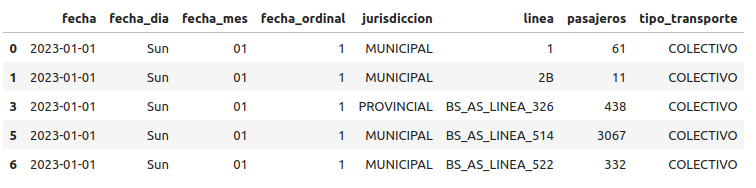
\includegraphics[width=\textwidth]{head.png}


\item Utilizando \verb|datos_amba|, identificar:
\begin{enumerate}
    \item la cantidad total anual de pasajeros para cada medio de transporte
    \item la línea de colectivos con la máxima cantidad de pasajeros para cada mes
    \item la fecha de menor movilidad promedio entre los colectivos de jurisdicción municipal.
\end{enumerate}

\item Elaborar un gráfico que permita comparar la media y los cuartiles de la cantidad de gente que viajó anualmente en cada una de las nueve líneas de colectivo que llegan a Ciudad Universitaria.

\item 


\end{enumerate}

\end{document}

